%%
%%% >>> Title Page
%%
%%
%%% Chinese Title Page
%%
  \confidential{}% show confidential tag
  \schoollogo{scale=0.45}{Img/UCAS}% university logo
  \title[兰州大学本科毕业设计实践~\LaTeX{}~模板]{全局和局部特征提取算法在人脸图像领域的比较}
  \author{栾英杰}% name of author
  \advisor{路永钢~教授}% names and titles of supervisors
  \advisorinstitute{兰州大学}% institute names of supervisors
  \degree{本科}% degree
  \degreetype{工学}% degree type
  \major{电子信息科学与工程}% major
  \institute{兰州大学}% institute of author
  %\chinesedate{2014~年~6~月}% only need for user customized date
%%
%%% English Title Page
%%

  \englishtitle{Facial Decomposition Methods Comparison \\ Between Global and Local Approaches }
  \englishauthor{Yingjie Luan}
  \englishadvisor{Professor Yonggang Lu}
  \englishdegree{Bachelor}
  \englishmajor{Engineering}
  \englishinstitute{School of Information Science and Technology,\\ Lanzhou University}
  %\englishdate{June, 2014}% only need for user customized date
%%
%%% Generate Chinese Title
%%
\maketitle
%%
%%% Generate English Title
%%
\makeenglishtitle
%%

%%
%%% >>> Abstract
%%
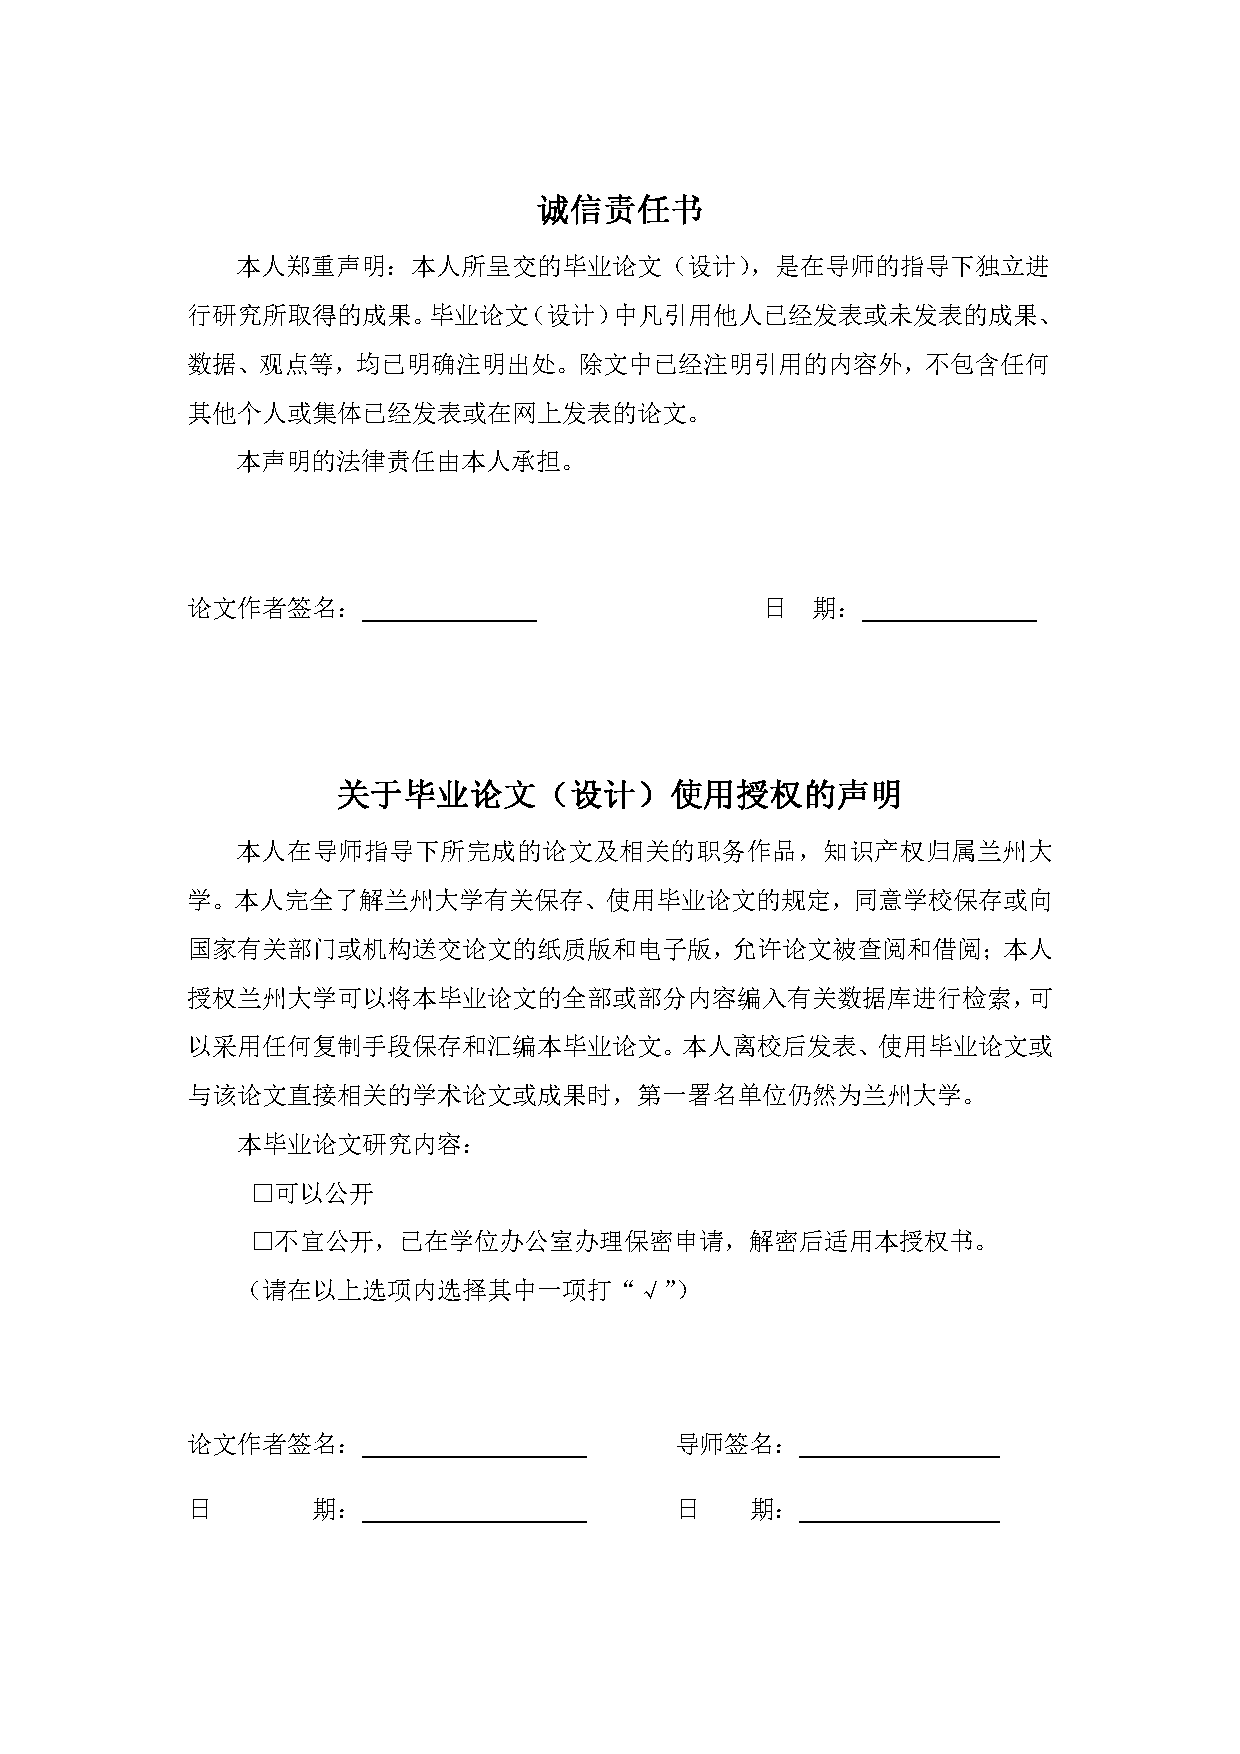
\includepdf{add1}

\begin{abstract}

本项目以人脸图片为主要内容,就不同降维算法的性能进行了比较,并尝试就实际人脸识别中的算法及参数选择问题给以一些建议.其主要内容有:

\paragraph{基于全局的特征提取算法} 本文首先实现了PCA, NMF, ICA等全局特征提取算法,这些算法有压缩率大,运行效率较高的优点,但也有着无法辨别背景,识别率存在上限的缺点.在对这些特征提取算法比较之后,作者发现比较难以实现精确的人脸识别,于是便开始了基于局部的特征提取算法的探究.
\paragraph{基于局部的特征提取算法} 本文以SIFT算子为例,实现了局部的特征提取算法.并对SIFT算子进行了一定的优化.SIFT相比较PCA算子,具有能区分背景,基于图像变换最大,信息最多的地方描述的优点.但是,也同时发现了SIFT算法计算速度较慢,内存占用大的缺点.
\paragraph{模型分析} 在实现上述内容的过程中,不可避免的出现了构建降维,分类等模型,并就模型的优劣进行比较.本项目也就机器学习中基本的模型比较过程进行了实践.



\keywords{本科课程实践,特征脸, 局部特征提取算法, 分类算法}
\end{abstract}


\begin{englishabstract}

The initial purpose of this project is to test the performance of different \textbf{Decomposition Algorithms} in terms of \textit{Facial Images}. PCA, NMF, ICA were implemented and has successfully compressed facial images with around 10,000 pixels into vectors of length 30 to 100. Besides that, a simple face recognition system was built with SVM as the classifier and the overall accuracy of successful recognition can be around 85\%. \newline

\textbf{Component-based approaches} were presented to conquer problems brought by the \textbf{global approach}. In comparison to global 
approaches, it only concentrates on the areas of images with the largest changes(or with maximum energy). And can provide a more accurate description of people. SIFT were implemented, and the overall accuracy can be 99\% at its maximum. \newline

Besides \textbf{global approach} and \textbf{component-based approaches}, this project also implemented  common frameworks for model evaluation. Both for the decomposition algorithms and classification algorithms.


\englishkeywords{Eigenfaces, Classification Algorithms, Component-based Feature Extraction, SIFT, Model Evaluation}
\end{englishabstract}
